\documentclass[12pt]{article}
\usepackage{graphicx}
\usepackage{fullpage}
\usepackage{verbatim}
\usepackage{caption}
\usepackage{float}
\usepackage[nottoc]{tocbibind} 
\usepackage{appendix}
\usepackage{titlesec}
\usepackage{tikz}
\usepackage{listings}
\usepackage{hyperref}
\hypersetup{
    colorlinks=true,
    linkcolor=blue,
    filecolor=magenta,      
    urlcolor=blue,
}
\usepackage[utf8]{inputenc}
\urlstyle{same}
\usetikzlibrary{shapes,arrows}
\titleformat{\chapter}[display]
  {\normalfont\bfseries}{}{0pt}{\Large}
  \usepackage[T1]{fontenc}
\usepackage[utf8]{inputenc}

  


\begin{document}
  \begin{titlepage}
    \begin{center}
      \begin{Large}
      \textbf{ Assignment- 10\\
       \vspace*{0.5cm}
       ELP - 718 Telecom Software Laboratory\\
       \vspace{1cm}
       Ch Krishna Chaitanya\\
       2019JTM2674\\
       2019-21\\}
      \end{Large}
       \vspace{1cm}
      {\Large  A report on Python with MySQL}
       \vfill
       \begin{figure}[h!]
          \centering
          
\includegraphics{iitdelhi.png}
       \end{figure}
       \vfill
      \begin{Large}
      \textbf{ Bharti School of \\
       Telecommunication Technology and Management\\
       IIT Delhi\\
       India\\
      }\end{Large}
       \medskip
       \today
    \end{center}
    \vfill
  \end{titlepage}
  
  \tableofcontents
  
  \clearpage
  \section*{Objective Statement}
   To test our understanding on implementation of mysql using python.

  \section{Problem Statement -1}
 To design a Database system for Restaurant Billing management which holds the details of customers on various days.

  \subsection{Problem Satement}
  
  \subsection{Algorithm and Implementation}
  \begin{itemize}
  \item Create Menu table with existing entries
  \item Create Bill table with no entries
  \item Design a menu for admin and customer
  \item For customer, display a menu
  \item Customer can chose items from menu
  \item Upon confirmation generate bill
  \item For admin, ask order number to dispaly respective order
  \item Admin can know bill amount in last n dayys by entering n
  \end{itemize}
  
  \subsection{Flowchart}
    % Define block styles
\tikzstyle{decision} = [diamond, draw, fill=blue!20, 
    text width=4.5em, text badly centered, node distance=3cm, inner sep=0pt]
\tikzstyle{block} = [rectangle, draw, fill=blue!20, 
    text width=6.5em, text centered, rounded corners, minimum height=3em]
\tikzstyle{line} = [draw, -latex']
\tikzstyle{cloud} = [draw, ellipse,fill=red!20, node distance=3cm,
    minimum height=3em]
\begin{center}    
\begin{tikzpicture}[node distance = 2cm, auto]
    % Place nodes
    
    \node [cloud] (init) {start};
    \node [block, below of=init] (First) {Create Menu, Bill tables};
    \node [block, below of=First] (Second) {Select 1.Customer 2.Admin};
    \node [decision, below of=Second] (Third) {If Customer?};
     \node [block, below of=Third,node distance=3cm] (Fouth) {Display Menu};
     \node [block, left of=Third,node distance=4cm] (Fifth) {Enetr Order number and days};
     
    \node [block, below of=Fifth,node distance=3cm] (Sixth) {Display Total Amount};
    \node [block, below of=Fouth,node distance=3cm] (Seventh) {Display Total Amount and Generate Bill};
    \node [cloud, below of=Sixth] (last_2) {stop};
    \node [cloud, below of=Seventh] (last_1) {stop};
  
    
    % Draw edges
    \path [line] (init) -- (First);
    \path [line] (First) -- (Second);
    \path [line] (Second) -- (Third);
     \path [line] (Third) -- node {yes}(Fouth);
     \path [line] (Fouth) --(Seventh);
     \path [line] (Seventh) --(last_1);
     \path [line] (Third) -- node{no}(Fifth);
     \path [line] (Fifth) --(Sixth);
     \path [line] (Sixth) --(last_2);
     
    
   
\end{tikzpicture}
\end{center}
  
 \newpage
  \subsection{Test Cases}
  
	\subsubsection{Input}
	Enter\\
1.Customer\\
2.Admin\\
\subsubsection{Output}
Select an option 1.Customer\\
2.Admin1\\
Enter Customer name : Krishna\\
Menu\\
(1, 'Idli', 30, 49)\\
(2, 'Dosa', 60, 40)\\
(3, 'Paneer Butter Masala', 130, 20)\\
(4, 'Tawa Roti', 8, 500)\\
(5, 'Fried Rice', 80, 100)\\
(6, 'Veg Thali', 100, 53)\\
(7, 'Wada Paav', 12, 3)\\
(8, 'Ice Tea', 50, 5)\\
(9, 'Cappuccino', 60, 33)\\
(10, 'Cafe Latte', 80, 29)\\
Enter Item Id\\
Item Available\\
Enter Quantity of Selected Item2\\
Idli 30\\
47\\
Do you eant to continue ?\\
1.Yes\\
2.Done1\\
Selected Items:\\
1, 'Idli', 30, 49\\
3, 'Paneer Butter Masala', 130, 20\\
The Total Amount is : 320\\
Do you want confirm order ?\\
1.Confirm\\
2.Edit1\\
order number  0001\\
\subsection{Screenshots}
\subsubsection{Screenshot1}
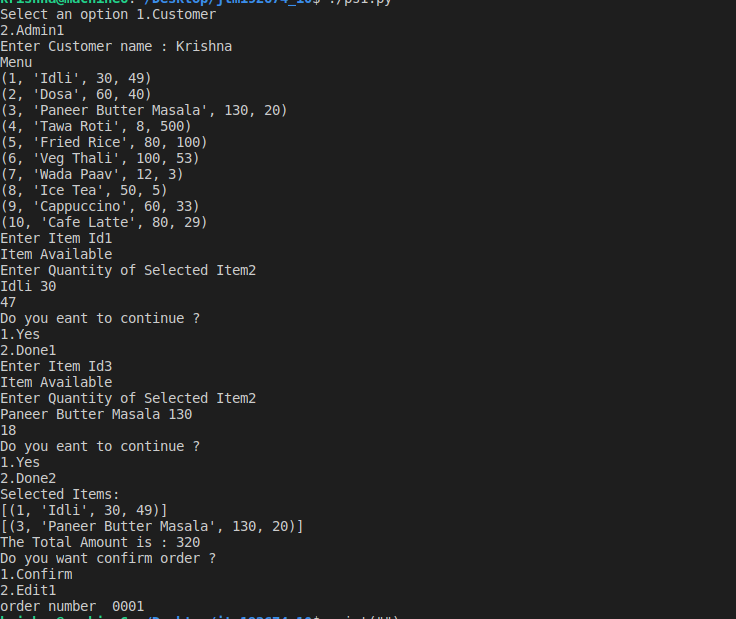
\includegraphics[width=\linewidth]{lab_10a.png}
\clearpage
\subsubsection{Screenshot2}
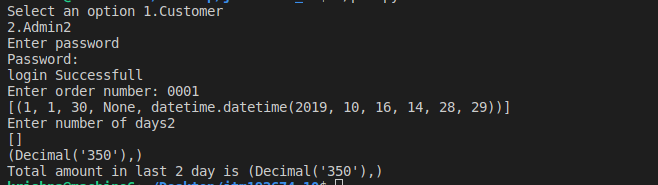
\includegraphics[width=\linewidth]{lab_10b.png}
\newpage
 \appendix
   \appendixpage
   \addappheadtotoc
  \section*{Problem 1}
  {\large \textbf{code:}}
  \verbatiminput{ps1.py}
  
\newpage
\begin{thebibliography}{11}
\bibitem{flowchart} 
Flowchart using Latex\\
Kjell Magne Fauske \\
\url{http://www.texample.net/tikz/examples/simple-flow-chart/}

\bibitem{Python Basics}
Python Basics \\
\url{https://docs.python.org/3/}

\bibitem{SQL}
SQL\\
\url{https://www.w3schools.com/sql/sql_groupby.asp}

\bibitem{PyMySQl}
PyMySQl\\
\url{http://zetcode.com/python/pymysql/}

\bibitem{MySQL using Python}
MySQL using Python\\
\url{https://www.w3schools.com/python/python_mysql_select.asp}

\end{thebibliography}

   
   
\end{document}
